% !TEX root = ../Ausarbeitung.tex
\newpage
\section{Aktuelle Lage}
\label{sec:AktuelleLage}
\Abbildung{Stats1} zeigt, dass trotz einiger Risiken der Container Technologie Unternehmen weltweit immer mehr Geld in die Containerisierung ihres Unternehmens investieren. Laut einer Umfrage, welche auf der DockerCon durchgeführt wurde, investierten 32\% der Unternehmen mindestens 500.000\$ jährlich, um die Containerisierung in ihrer Organisation voranzutreiben. \cite{Investments}
\begin{figure}[H]
	\begin{center}
		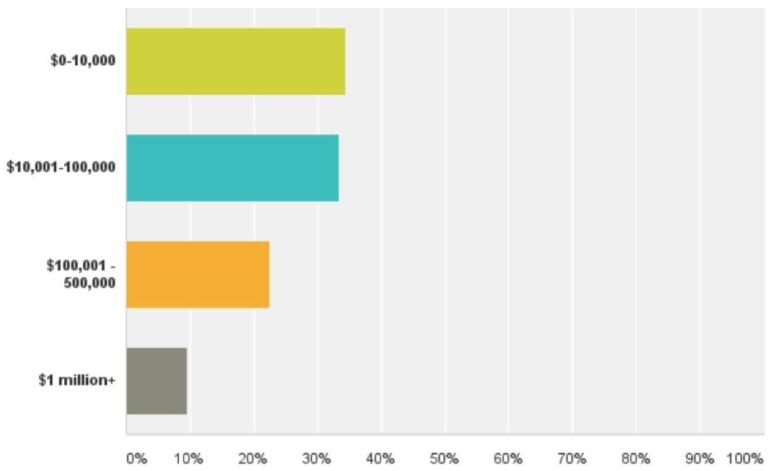
\includegraphics[width=0.8\textwidth]{ContainerInvest.png}
	\end{center}
	\caption[Investitionen in die Containerisierung]{Investitionen in die Containerisierung \footnotemark}
	\label{fig:Stats1}
\end{figure}
\quellefoot{https://portworx.com/wp-content/uploads/2017/04/survey-investment-768x471.png}
\newpage
Aus \Abbildung{Stats2} ist zu entnehmen, dass 83\% der produktiv eingesetzten Container von Docker stammen. An zweiter Stelle der meist verwendeten Container findet sich CoreOS, welches von der Firma Red Hat übernommen wurde. Mesos Containerizer und Linux Containers (LXC) machen zusammen nur 5\% aller eingesetzten Container aus.
\begin{figure}[H]
	\begin{center}
		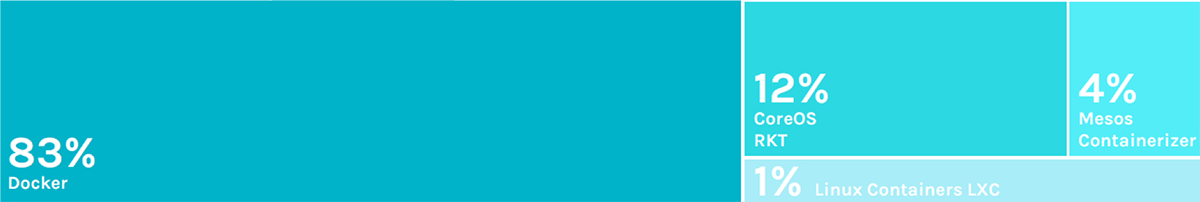
\includegraphics[width=1.1\textwidth]{DockerProzent.png}
	\end{center}
	\caption[Benutzung von Containertechnologien]{Benutzung von Containertechnologien \footnotemark}
	\label{fig:Stats2}
\end{figure}
\quellefoot{https://www.dailyhostnews.com/wp-content/uploads/2018/05/d2.png}
Laut eines Berichts der Container-Monitoring-Firma Sysdig stieg die Anzahl der durchschnittlich verwendeten Container pro Host 2018 um 50\% im Vergleich zum Vorjahr. Das entspricht nun etwa 15 Containern. Laut des Berichts ist 154 die maximale Anzahl von Containern, die bisher gleichzeitig auf einer Maschine laufen. \Abbildung{Stats3} stellt dies grafisch dar.
\begin{figure}[H]
	\begin{center}
		
\includegraphics[width=0.8\textwidth]{ContainerHost.png}
	\end{center}
	\caption[Container je Maschine]{Container je Maschine \footnotemark}
	\label{fig:Stats3}
\end{figure}
\quellefoot{https://www.dailyhostnews.com/wp-content/uploads/2018/05/d1.png}
\newpage
Kubernetes sei die meist genutzte Plattform, um Container zu orchestrieren und wird von Software-Unternehmen wie Microsoft und IBM verwendet. Das beliebteste Tool, um Container-Cluster für große Firmen auszurollen, sei jedoch Mesos Containerizer. \cite{stats} Die genaue Verteilung ist \Abbildung{Stats4} zu entnehmen.
\begin{figure}[H]
	\begin{center}
		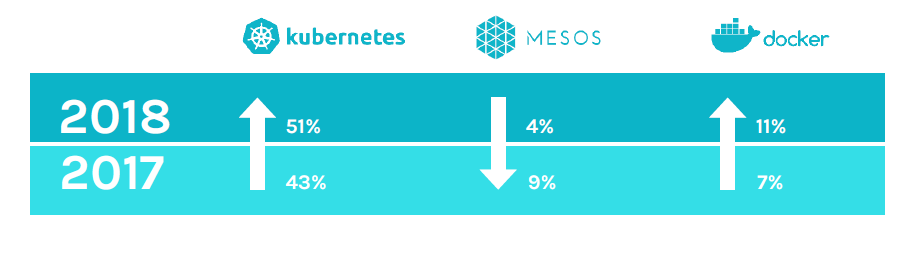
\includegraphics[width=0.8\textwidth]{Manager.png}
	\end{center}
	\caption[Cluster-Manager]{Cluster-Manager \footnotemark}
	\label{fig:Stats4}
\end{figure}
\quellefoot{https://www.dailyhostnews.com/wp-content/uploads/2018/05/d4.png}

